\documentclass[conference]{IEEEtran}
\usepackage[T1]{fontenc}
\usepackage[utf8]{inputenc}
\usepackage{helvet}
\usepackage{courier}
\usepackage{amssymb}
\usepackage{xcolor}
\usepackage{array}
\usepackage{booktabs}
\usepackage{tikz}
\usetikzlibrary{shapes.geometric,arrows.meta,positioning,fit,backgrounds,calc}
\usepackage{cite}
\usepackage{microtype}

% ==== figure palette: three hues plus greys, separated by value in greyscale
\definecolor{agF}{HTML}{F6F2FC}\definecolor{agB}{HTML}{6B4FA0} % agent, violet
\definecolor{rbF}{HTML}{A9C4DC}\definecolor{rbB}{HTML}{2F6FAF} % apparatus, blue
\definecolor{dsF}{HTML}{DCDCE0}\definecolor{dsB}{HTML}{9A9AA0} % discarded, grey
\definecolor{hgB}{HTML}{3E6B52}                                % human, green
\definecolor{dgrey}{HTML}{555555}\definecolor{fgrey}{HTML}{7A7A7A}

\begin{document}

\title{Seed, Generate, Reduce, Repair, Gate:\\A Closed CIRCT Bug Loop}

\author{\IEEEauthorblockN{Abhinav Venkata Kota, Adithya Jillellamudi, Priyesh Shukla}
\IEEEauthorblockA{International Institute of Information Technology, Hyderabad\\
\{abhinav.kota, adithya.jillellamudi\}@students.iiit.ac.in, priyesh.shukla@iiit.ac.in}}

\maketitle

\begin{abstract}
CIRCT is an open-source compiler that turns hardware descriptions into Verilog,
the text that chip design tools consume, so a defect inside it can corrupt a
design unnoticed. Agents that repair CIRCT take their work from its public issue
tracker, a queue users fill and maintainers, whose attention is the scarce
resource, must drain. We describe a loop that makes its own supply: an agent
reads a past bug fix, states the class of mistake it corrected, and writes fresh
inputs probing for the same mistake elsewhere in the compiler. A fixed harness
then builds, judges, minimises, deduplicates and repairs, and a gate ending in
human approval decides what, if anything, is filed. We evaluate the seeded agent
against a mutation fuzzer at equal, pre-registered budget under identical tools.
We release the loop as reusable nodes and tools for the CHIA agent framework,
with its seed corpus, transcripts and verdicts.
\end{abstract}

% =====================================================================
\section{Introduction}
CIRCT is an open-source compiler for hardware. A designer writes how a circuit
should behave, in FIRRTL (the form the Chisel hardware language produces) or in
SystemVerilog, and CIRCT lowers it to Verilog, the text that synthesis and
layout tools turn into a chip. It is built on MLIR, the LLVM project's framework
for assembling a compiler out of interchangeable intermediate languages, and it
inherits LLVM's way of testing: each regression test is a file carrying the
exact command to run and the output pattern to expect, executed by a runner
called \texttt{lit}.

A CIRCT bug that crashes the compiler is an inconvenience: the designer sees it and works around it. A bug that makes CIRCT emit wrong Verilog is not, because the output is well formed, passes the tools below it, and can reach fabrication unnoticed.

CHIA \cite{chia} is the agent framework this hackathon is built on. An agent
here is a language model wired into a program that reads files, runs commands
and decides what to do next. CHIA ships an issue solver for CIRCT that chains
six phases: assess the issue, reproduce it with a script, fix it, verify by rebuilding and rerunning the whole test suite, repair any regression the fix caused, and write the pull request description. Run on 16 CIRCT issues
it fixed five, and three of those became merged pull requests. It writes nothing
to GitHub; both of its flows only read.

Its supply is the constraint. Over the past year CIRCT received 82 issues labelled as bugs and closed 65, so the project is neither short of reports nor ignoring them. What does not happen is the backlog draining: 101
bug-labelled issues are open, at a median age of 911 days. The scarce resource
is maintainer attention, not bug supply, and an agent that empties the queue
faster creates none. What would help is a bug that arrives already minimised,
already checked against what is known, already carrying a candidate fix, from a
source that files nothing else.

Past fixes are unspent information. A commit that corrects one wrong assumption
inside a compiler pass usually leaves the same assumption standing at other
sites, and CIRCT ships no fuzzing infrastructure in its own tree to find them.

This paper describes a loop that manufactures its own supply and then withholds
most of it. We contribute the loop design (Section~\ref{sec:loop}), two preconditions we measured and repaired before it could run
(Section~\ref{sec:pre}), and a pre-registered head-to-head against a mutation
fuzzer (Section~\ref{sec:eval}).

\begin{figure*}[!t]
\centering
% fig-loop.tex -- full-width figure: the attrition ribbon.
% Absolute coordinates in cm. Canvas: x 0.00..18.10, y 1.65..10.70.
% The ribbon's top edge is constant at y=5.50. Its thickness drops at each gate
% and the lost slice peels away downward onto the floor at y=2.50.
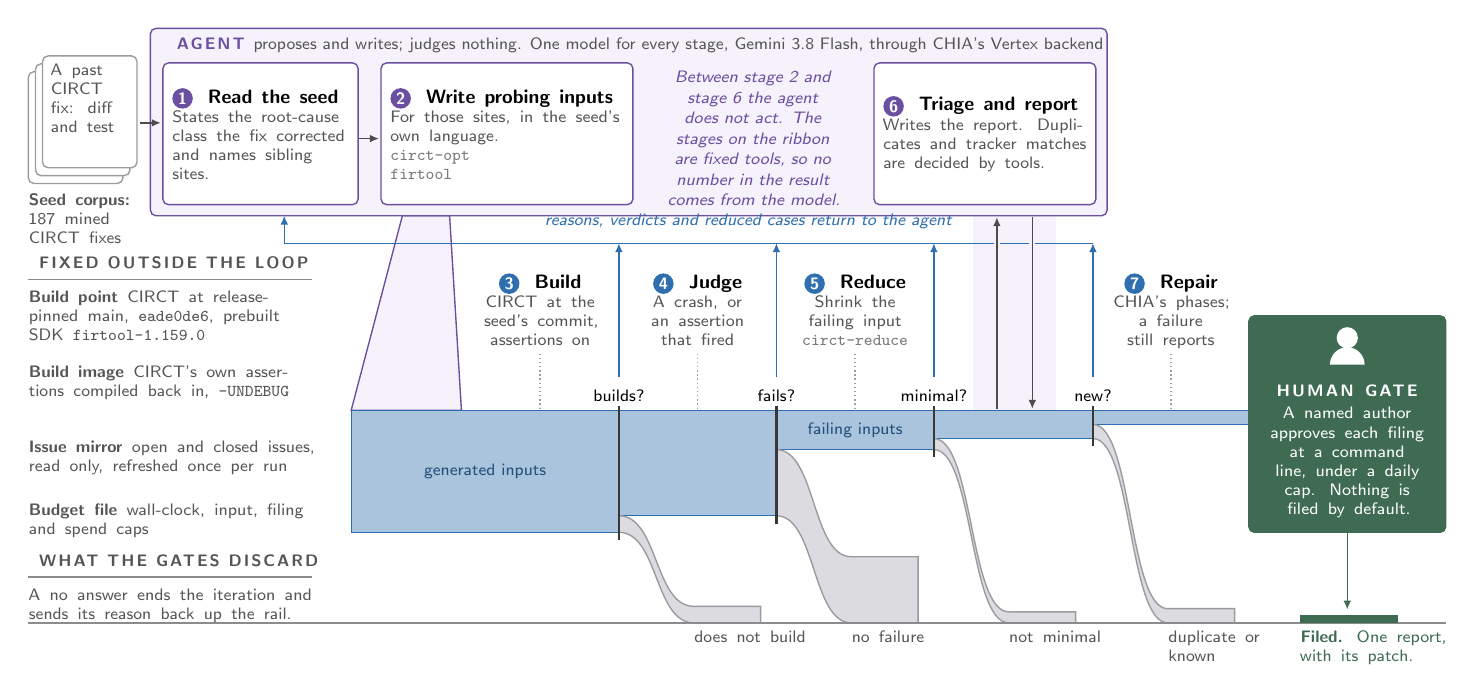
\begin{tikzpicture}[x=1cm,y=1cm,
  font=\sffamily,
  card/.style={draw=agB, fill=white, line width=0.5pt, rounded corners=2pt,
               anchor=north west, align=left, inner xsep=3.4pt, inner ysep=3.4pt},
  blk/.style={anchor=north, align=center, inner sep=1pt},
  txt/.style={anchor=north west, align=left, inner sep=0pt},
  hair/.style={line width=0.5pt, draw=black!45},
  rail/.style={line width=0.5pt, draw=rbB},
  arr/.style={-{Latex[length=3.2pt,width=2.8pt]}, line width=0.5pt, draw=black!70},
  rarr/.style={-{Latex[length=3.2pt,width=2.8pt]}, line width=0.5pt, draw=rbB},
  gatemark/.style={line width=1.0pt, draw=black!78},
  ]

% === type helpers
\newcommand{\ct}[1]{{\sffamily\bfseries\fontsize{7}{7.9}\selectfont #1\par}}
\newcommand{\cd}[1]{{\sffamily\fontsize{6}{6.9}\selectfont\color{dgrey}#1\par}}
\newcommand{\cm}[1]{{\ttfamily\fontsize{6}{6.9}\selectfont\color{fgrey}#1\par}}
\newcommand{\hdr}[1]{{\sffamily\bfseries\fontsize{6.2}{7.2}\selectfont\textls[110]{#1}}}
\newcommand{\lab}[1]{{\sffamily\fontsize{6}{6.9}\selectfont #1}}
\newcommand{\rlab}[1]{{\sffamily\fontsize{6}{6.9}\selectfont\color{rbB!70!black}#1}}
\newcommand{\nm}[2]{\tikz[baseline=(n.base)]{\node[circle,fill=#2,inner sep=0pt,
   minimum size=7.4pt,anchor=base](n){\textcolor{white}{\sffamily\bfseries
   \fontsize{6}{6}\selectfont\raisebox{-0.4pt}{#1}}};}}
\newcommand{\fx}[4]{\node[txt, text width=3.60cm]
  at (#1,#2) {\cd{\textbf{#3}\ #4}};}

% =============================================== where the agent reaches the flow
% funnel: stage 2 pours generated inputs into the ribbon
\fill[agF, draw=agB, line width=0.5pt]
  (4.80,7.97) -- (5.40,7.97) -- (5.55,5.50) -- (4.15,5.50) -- cycle;
% shaft: the flow rises into stage 6 and comes back down
\fill[agF] (12.05,5.50) rectangle (13.10,7.97);

% ================================================================== agent band
\draw[fill=agF, draw=agB, line width=0.5pt, rounded corners=2pt]
  (1.60,7.97) rectangle (13.75,10.35);
\node[anchor=base west] at (1.80,10.08)
  {{\color{agB}\hdr{AGENT}}\;{\sffamily\fontsize{6.2}{7.2}\selectfont
   \color{dgrey}proposes and writes; judges nothing. One model for every stage,
   Gemini 3.8 Flash, through CHIA's Vertex backend}};
% model and backend: design/ADR/ADR-D-03-model-backend.md, superseding decision 2026-09-14

\node[card, text width=2.24cm, minimum height=1.80cm] at (1.75,9.92)
  {\ct{\nm{1}{agB}\; Read the seed}\cd{States the root-cause class the fix
   corrected and names sibling sites.}};
\node[card, text width=2.96cm, minimum height=1.80cm] at (4.52,9.92)
  {\ct{\nm{2}{agB}\; Write probing inputs}\cd{For those sites, in the seed's own language.}\cm{circt-opt}\cm{firtool}};
\node[card, text width=2.58cm, minimum height=1.80cm] at (10.78,9.92)
  {\ct{\nm{6}{agB}\; Triage and report}\cd{Writes the report. Duplicates and
   tracker matches are decided by tools.}};

\draw[arr] (4.25,8.95) -- (4.50,8.95);

\node[anchor=center, text width=2.42cm, align=center, color=agB,
      font=\sffamily\itshape\fontsize{6.2}{7.4}\selectfont] at (9.25,8.95)
  {Between stage 2 and stage 6 the agent does not act. The stages on the ribbon
   are fixed tools, so no number in the result comes from the model.};

% ================================================================= seed corpus
\foreach \i in {0,1,2}
  {\draw[fill=white, draw=dsB, line width=0.5pt, rounded corners=2pt]
     (0.05+0.09*\i,8.38+0.10*\i) rectangle +(1.20,1.42);}
\node[txt, text width=0.98cm] at (0.33,9.91)
  {\cd{A past CIRCT fix: diff and test}};
\node[txt, text width=1.62cm] at (0.05,8.25)
  {\cd{\textbf{Seed corpus:} 187 mined CIRCT fixes}};
\draw[arr] (1.47,9.15) -- (1.73,9.15);

% ================================================================= return rail
\draw[rail] (13.57,7.62) -- (3.30,7.62);
\draw[rarr] (3.30,7.62) -- (3.30,7.97);
\node[anchor=south east, color=rbB,
      font=\sffamily\itshape\fontsize{6}{7}\selectfont] at (11.90,7.68)
  {reasons, verdicts and reduced cases return to the agent};

% ============================================================ apparatus stages
\node[blk, text width=1.58cm] at (6.55,7.28)
  {\ct{\nm{3}{rbB}\; Build}\cd{CIRCT at the seed's commit, assertions on}};
\node[blk, text width=1.58cm] at (8.55,7.28)
  {\ct{\nm{4}{rbB}\; Judge}\cd{A crash, or an assertion that fired}};
\node[blk, text width=1.58cm] at (10.55,7.28)
  {\ct{\nm{5}{rbB}\; Reduce}\cd{Shrink the failing input}\cm{circt-reduce}};
\node[blk, text width=1.58cm] at (14.56,7.28)
  {\ct{\nm{7}{rbB}\; Repair}\cd{CHIA's phases; a failure still reports}};

\foreach \x in {6.55,8.55,10.55,14.56}
  {\draw[line width=0.5pt, draw=black!38, densely dotted] (\x,6.22) -- (\x,5.52);}

% ======================================================================= ribbon
% segment: from, to, thickness below the constant top edge y=5.50
\foreach \a/\b/\h in {4.15/7.55/1.55, 7.55/9.55/1.34, 9.55/11.55/0.50,
                      11.55/13.57/0.36, 13.57/15.55/0.18}
  {\fill[rbF] (\a,5.50) rectangle (\b,5.50-\h);
   \draw[line width=0.5pt, draw=rbB] (\a,5.50) -- (\b,5.50);
   \draw[line width=0.5pt, draw=rbB] (\a,5.50-\h) -- (\b,5.50-\h);}
\draw[line width=0.5pt, draw=rbB] (4.15,5.50) -- (4.15,3.95);

% what is in flight, named where the ribbon is tall enough to hold the words
\node[anchor=center, inner sep=0pt] at (5.85,4.72) {\rlab{generated inputs}};
\node[anchor=center, inner sep=0pt] at (10.55,5.25) {\rlab{failing inputs}};

% stage 6: the flow rises into the agent and comes back
\draw[arr, preaction={draw, line width=2.2pt, agF}] (12.35,5.52) -- (12.35,7.95);
\draw[arr, preaction={draw, line width=2.2pt, agF}] (12.80,7.95) -- (12.80,5.52);

% ======================================================== gates and what they shed
% gate x, ribbon bottom before, ribbon bottom after, the question
\foreach \g/\bo/\bn/\q in {7.55/3.95/4.16/builds?, 9.55/4.16/5.00/fails?,
                           11.55/5.00/5.14/minimal?, 13.57/5.14/5.32/new?}
  {\fill[dsF, draw=dsB, line width=0.5pt]
     (\g,\bn) .. controls (\g+0.50,\bn) and (\g+0.45,2.80+\bn-\bo) ..
     (\g+0.95,2.80+\bn-\bo) -- (\g+1.80,2.80+\bn-\bo) -- (\g+1.80,2.80)
     -- (\g+0.95,2.80) .. controls (\g+0.45,2.80) and (\g+0.50,\bo) ..
     (\g,\bo) -- cycle;
   \draw[gatemark] (\g,\bo-0.10) -- (\g,5.56);
   \node[anchor=south, inner sep=0.7pt, fill=white] at (\g,5.58) {\lab{\q}};
   \draw[rarr] (\g,5.92) -- (\g,7.62);}

\foreach \g/\l in {7.55/does not build, 9.55/no failure,
                   11.55/not minimal, 13.57/duplicate or known}
  {\node[txt, text width=1.50cm] at (\g+0.95,2.70)
     {\cd{\l}};}

% ======================================================== fixed outside the loop
\node[anchor=base west, color=dgrey] at (0.05,7.30) {\hdr{FIXED OUTSIDE THE LOOP}};
\draw[hair] (0.05,7.16) -- (3.65,7.16);
% build point eade0de6 with SDK firtool-1.159.0: analysis/measurements/2026-09-14-image-build.md 1
\fx{0.05}{7.02}{Build point}{CIRCT at release-pinned main, \texttt{eade0de6}, prebuilt SDK \texttt{firtool-1.159.0}}
\fx{0.05}{6.07}{Build image}{CIRCT's own assertions compiled back in, \texttt{-UNDEBUG}}
\fx{0.05}{5.12}{Issue mirror}{open and closed issues, read only, refreshed once per run}
\fx{0.05}{4.32}{Budget file}{wall-clock, input, filing and spend caps}

% ======================================================================== floor
\draw[hair] (0.05,2.80) -- (18.05,2.80);
\node[anchor=base west, color=dgrey] at (0.05,3.52) {\hdr{WHAT THE GATES DISCARD}};
\draw[hair] (0.05,3.38) -- (3.65,3.38);
\node[txt, text width=3.60cm] at (0.05,3.24)
  {\cd{A no answer ends the iteration and sends its reason back up the rail.}};

% =================================================================== human gate
\draw[fill=hgB, draw=hgB, line width=0.5pt, rounded corners=2pt]
  (15.55,3.95) rectangle (18.05,6.70);
\fill[white] (16.80,6.42) circle (0.135);
\fill[white] (16.58,6.08) arc[start angle=180, end angle=0, radius=0.22] -- cycle;
\node[anchor=north, text width=2.22cm, align=center, color=white] at (16.80,5.94)
  {\hdr{HUMAN GATE}};
\node[anchor=north, text width=2.22cm, align=center, color=white] at (16.80,5.66)
  {{\sffamily\fontsize{6}{6.9}\selectfont A named author approves each filing at
   a command line, under a daily cap. Nothing is filed by default.\par}};

\draw[arr, draw=hgB] (16.80,3.95) -- (16.80,2.97);
\fill[hgB] (16.20,2.80) rectangle (17.45,2.90);
\node[txt, text width=1.85cm] at (16.20,2.70)
  {{\sffamily\fontsize{6}{6.9}\selectfont\color{hgB}\textbf{Filed.} One report,
   with its patch.\par}};

\end{tikzpicture}

\caption{Seeded CIRCT bug loop, a CHIA loop for turning past fixes into new,
checked, repair-carrying bug reports. The agent holds the violet band at the
top and acts three times only, at stages 1, 2 and 6; the blue ribbon below it is
fixed apparatus, so no number in the result comes from the model. The ribbon is
the candidates in flight. It is poured wide out of stage 2 and pinched by a bar
at each gate, a question with two answers: the share answering no peels away
onto the floor and ends its iteration, the rest carries on, and the reason
climbs the thin rail back to the agent. Only a sliver survives to the human
gate, which files nothing without a named author's approval. Ribbon and peel
widths are illustrative, not measured.}
\label{fig:loop}
\end{figure*}

% =====================================================================
\section{The Loop}\label{sec:loop}
Fig.~\ref{fig:loop} names the stages and marks the ones the agent runs. The
agent proposes inputs and writes prose; the tools decide everything else, so no number in the result comes from inside the model.

\textbf{Read the seed (1).} A seed is one of 187 CIRCT commits from the last two
years that look like bug fixes, each with its diff and the test its author added
or changed. The agent reads both, states in one sentence the root-cause class
the fix corrected, and names other sites in the compiler where the same
assumption still stands.

\textbf{Write probing inputs (2).} The seed's own test decides the language of
the new inputs. Its command line names the tool through which the bug was
reachable: \texttt{circt-opt}, which runs a named sequence of compiler passes
over an intermediate file; \texttt{firtool}, the end-to-end driver from FIRRTL
to Verilog; or the SystemVerilog front end. About 127 of the 187 seeds sit in
code that no FIRRTL input can reach, so a generator that emitted only FIRRTL
would be blind to most of the corpus.

\textbf{Build (3).} CIRCT compiles against one pinned commit of LLVM and MLIR,
and building those from source costs hours; Section~\ref{sec:pre} explains how
the loop avoids that. The build also compiles in CIRCT's assertions, the
internal consistency checks its own authors wrote into the source, which stop
the compiler the moment an assumption breaks instead of letting the damage
travel into the output.

\textbf{Judge (4).} An oracle is the rule that decides whether an input has
found a bug. The primary one admits no argument: the compiler crashed, or one of
its assertions fired. A second oracle runs the same design through CIRCT's
simulator and through Verilator, an independent and long-established one, and
treats disagreement as suspicious. It produces reports only, because the two
disagree routinely over uninitialised and reset signals.

\textbf{Reduce (5).} An input that triggers a crash is usually large and mostly
irrelevant to it. Reduction is the mechanical search for a smaller input that
still fails: \texttt{circt-reduce}, which CIRCT ships, deletes parts of the
input and keeps each deletion while the failure survives. A maintainer then reads the case in a minute, not an hour.

\textbf{Triage and report (6).} Many failures are one failure. Deduplication
decides which candidates are the same bug, by assertion text and source
location, by symbolised stack frames, and by a structural hash of the reduced
input. Survivors are checked against CIRCT's open and closed issues and the commits made since the build point. The agent classifies each survivor as a
bug, an invalid input or a known issue, and writes the report a maintainer would
read.

\textbf{Repair (7).} CHIA's phase chain runs unaltered; the only addition is an entry point that accepts a local report in place of a GitHub issue. Repair is
restricted to crashes and assertion failures, where nobody has to argue about
what the right answer was.

\textbf{The gates.} Between stages sit questions with two answers, drawn as the
bars that pinch the ribbon in Fig.~\ref{fig:loop}: does it build, does it fail,
is it minimal, is it new. A no ends the iteration, skips every stage downstream of it, and returns
the reason to the agent with the oracle verdicts and reduced cases. The last
gate is a person. A named author approves every filing, under a cap on filings
per day, and the loop files nothing by default.

\begin{table}[!t]
\caption{What we measured, and what it means}
\label{tab:meas}
\centering
\scriptsize
\renewcommand{\arraystretch}{1.12}
\begin{tabular}{@{}>{\raggedright\arraybackslash}p{2.55cm}@{\hspace{5pt}}>{\raggedright\arraybackslash}p{1.42cm}@{\hspace{5pt}}>{\raggedright\arraybackslash}p{3.62cm}@{}}
\toprule
\textbf{Measurement} & \textbf{Result} & \textbf{What it means} \\
\midrule
\multicolumn{3}{@{}l}{\textit{Building CIRCT at a past commit}}\\
Fix-shaped commits mined from 24 months & 187 & The seed corpus: each is a past bug with its fix and its test. \\
Seeds with an exactly matching prebuilt SDK & 171 & Nearly all of them rebuild in minutes rather than hours. \\
One full build, assertions off, \texttt{circt-opt} targets only & 1{,}027 targets, 939\,s & Cheap enough to redo per seed. The seed's test was red before its fix and green after. \\
Pin windows with no matching release & 16 of 63 & Sometimes no buildable point exists. The worst run lasted 100 commits and 16 days. \\
Lag from a pin change to a usable release & 3.3\,d median, 33.5\,d worst & The loop's build point trails the branch head by days. \\
\addlinespace[2pt]
\multicolumn{3}{@{}l}{\textit{Letting the compiler complain}}\\
Compile commands defining \texttt{NDEBUG} & 620 of 620 & Assertions are absent from the stock CHIA image. \\
Assertion-handler references in the built binary & 0 & The primary oracle would have nothing to detect. \\
Targets that build with \texttt{-UNDEBUG} & 605 of 605 & Restoring the assertions does not break the build. \\
Object files carrying the handler again & 495 of 513 & The checks are back across the compiler. \\
Core dialect and conversion tests passing with assertions on & 520 of 523 & CIRCT still behaves. The three failures trace to a stale SDK tool. \\
\bottomrule
\end{tabular}
\end{table}

% =====================================================================
\section{Two Measured Preconditions}\label{sec:pre}
The loop has to build CIRCT at arbitrary points of its history, and the compiler
has to be able to complain. Neither held when we started. Table~\ref{tab:meas}
lists what we measured, and this section gives the conclusions.

\subsection{Building the past cheaply}
CIRCT records the exact LLVM commit it expects, called the pin, and a build against any other fails outright rather than degrading, stopping in the first few targets. Compiling that LLVM from source costs hours per seed and would consume the campaign's budget. The project also publishes release tarballs of prebuilt LLVM and MLIR libraries, an SDK, each recording the pin it was built against. Where a release shares a seed's pin, CIRCT rebuilds in minutes. We mined 187 fix-shaped commits from 24 months
of history and found an exactly matching SDK for 171 of them. To check that the
mechanism works rather than merely counts, we rebuilt one seed from a stock release: its own test failed at the commit before the fix and passed at the fix.

\begin{figure}[!t]
\centering
% fig-timeline.tex -- single-column timeline explaining release-pinned main.
% Canvas: x 0..8.7, y 0.5..3.2 (cm).
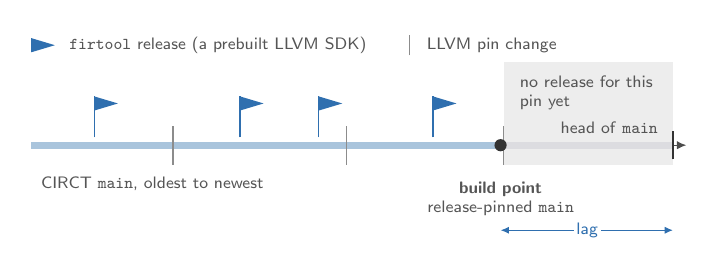
\begin{tikzpicture}[x=1cm,y=1cm, font=\sffamily,
  tiny/.style={font=\sffamily\fontsize{6}{6.8}\selectfont, color=dgrey},
  tick/.style={line width=0.5pt, draw=black!45},
  ]

% === legend row
\draw[line width=0.5pt, draw=rbB] (0.30,2.98) -- (0.30,3.16);
\fill[rbB] (0.30,3.16) -- (0.60,3.07) -- (0.30,2.98) -- cycle;
\node[tiny, anchor=west] at (0.66,3.07) {\texttt{firtool} release (a prebuilt LLVM SDK)};
\draw[tick] (5.10,2.94) -- (5.10,3.20);
\node[tiny, anchor=west] at (5.20,3.07) {LLVM pin change};

% === window with no release yet
\fill[black!7] (6.30,1.55) rectangle (8.45,2.86);
\node[tiny, anchor=north west, text width=2.00cm, align=left] at (6.38,2.80)
  {no release for this pin yet};

% === the branch, one colour per pin window
\draw[line width=2.6pt, draw=rbF] (0.30,1.80) -- (2.10,1.80);
\draw[line width=2.6pt, draw=rbF] (2.10,1.80) -- (4.30,1.80);
\draw[line width=2.6pt, draw=rbF] (4.30,1.80) -- (6.30,1.80);
\draw[line width=2.6pt, draw=dsF] (6.30,1.80) -- (8.45,1.80);
\draw[-{Latex[length=3.4pt,width=3pt]}, line width=0.5pt, draw=black!70]
  (8.45,1.80) -- (8.62,1.80);
\node[tiny, anchor=north west] at (0.30,1.52) {CIRCT \texttt{main}, oldest to newest};

% === pin changes
\foreach \x in {2.10,4.30,6.30} {\draw[tick] (\x,1.55) -- (\x,2.05);}

% === releases
\foreach \x in {1.10,2.95,3.95,5.40} {
  \draw[line width=0.5pt, draw=rbB] (\x,1.90) -- (\x,2.42);
  \fill[rbB] (\x,2.42) -- (\x+0.30,2.33) -- (\x,2.24) -- cycle;}

% === build point and head
\fill[black!80] (6.26,1.80) circle (2.2pt);
\node[tiny, anchor=north, text width=2.3cm, align=center] at (6.26,1.46)
  {\textbf{build point}\\release-pinned \texttt{main}};
\draw[line width=1.0pt, draw=black!80] (8.45,1.62) -- (8.45,1.98);
\node[tiny, anchor=north east] at (8.38,2.22) {head of \texttt{main}};

% === lag
\draw[{Latex[length=3pt,width=2.6pt]}-{Latex[length=3pt,width=2.6pt]},
      line width=0.5pt, draw=rbB] (6.26,0.72) -- (8.45,0.72);
\node[tiny, color=rbB, fill=white, inner sep=1pt] at (7.36,0.72) {lag};

\end{tikzpicture}

\caption{Release-pinned \texttt{main}. Changes to the LLVM commit CIRCT pins cut
its branch into windows, and a prebuilt SDK exists for a window only where a
release falls inside it. The loop builds at the newest commit whose pin has a
release, which is the head of the branch only while the current window has one.
A bug fixed inside the lag is found again by the loop and dropped as already
known.}
\label{fig:timeline}
\end{figure}

The same mechanism fixes where the loop runs. It does not run at the newest commit of CIRCT's main branch, whose pin has no published release today. It runs at release-pinned main, the newest commit whose pin does
have one. That point trails the branch head by days, as Fig.~\ref{fig:timeline} shows.

\subsection{Letting the compiler complain}
Optimised builds delete assertions by defining the macro \texttt{NDEBUG}. CHIA's
CIRCT image is such a build: every one of its 620 compile commands defines that
macro, and the resulting binary holds no reference to the assertion handler at
all. A loop whose primary oracle is a failed assertion would find nothing under
the stock image, whatever the agent wrote. One compiler flag,
\texttt{-UNDEBUG}, puts the assertions back. The build still completes, nearly
every object file carries the handler again, and the core dialect and conversion
tests still pass on all but three, which fail for an unrelated reason (a stale tool in the SDK). The restored binary still describes itself as an optimised
build, so every report the loop files has to name the flag.

One caution about Table~\ref{tab:meas}: the timed build was made with assertions
off and covered only one of CIRCT's tools, so it is a lower bound
on what the loop's image will cost.

% =====================================================================
\section{Evaluation Design}\label{sec:eval}
The experiment asks whether reading a past fix makes an agent better at finding
new bugs than mutating the same tests at random. Two arms run the same harness, oracles, reducer and gate; only the generator differs. The seeded arm is stages 1 and 2 above. The mutation arm starts from
the same seed tests and applies syntactic mutations without ever seeing the diff
or the root-cause class, following Mut4All's design for mutators synthesised by
a language model \cite{mut4all}.

Both arms spend the same pre-registered budget: the compute allowance and the caps on generated inputs and on filings are committed to the public loop repository before the campaign starts, so no threshold can be chosen afterwards. The headline result is the number of distinct bugs a
CIRCT maintainer confirmed, by labelling, commenting on or fixing them, within
that budget. Our own oracle agreeing with itself produces a candidate, not a
bug. The secondary counts are candidates before and after deduplication, reports
filed, the fraction of filed reports maintainers accepted, and repairs merged.

If both arms find nothing, the paper reports that. Pre-registration is what
makes such an outcome publishable, and it carries information: CIRCT's assertion
surface would not be reachable at this budget by either strategy.

\textbf{Contamination.} CIRCT's history is public and sits in the training data
of any model we can use, so the agent may reproduce a fix it memorised. Every candidate is screened against fixes made after
its seed, and a match is recorded and reported apart from the rest. A match does
not make the candidate invalid, since a real crash is a real crash, but it
changes what the number means. The repair stage runs CHIA's executor unchanged
and is not screened.

\textbf{Maintainer protocol.} We post the method to the project's forum before
the campaign starts, and leave issues marked as good first issues to human
newcomers.

\textbf{Failure taxonomy.} Every candidate reaching the gate is recorded with its verdict, one of unreproducible, not minimal, invalid input, duplicate, undecided or new bug,
and every repair attempt with the phase that failed. The record shows where the
loop spent budget without return.

% =====================================================================
\section{Related Work}
\textbf{Agentic repair.} SWE-bench \cite{swebench} scores agents on real GitHub
issues and set the pattern this work inherits; CHIA's issue solver \cite{chia} applies it to a hardware compiler. Both draw from a queue; we add the stage that fills one.

\textbf{Compiler fuzzing.} CSmith \cite{csmith} generates random C programs and found previously unknown bugs throughout production C compilers. For MLIR, the framework CIRCT is built
on, MLIRod mutates along operation dependencies \cite{mlirod}, N\"uwa adds
generation driven by a language model \cite{nuwa}, DESIL targets silent
wrong-output bugs \cite{desil}, and FLEX interleaves learning with exploration
and found 80 previously unknown bugs in a 30-day campaign \cite{flex}. None of
them repairs or withholds; they hand a
human a pile of crashes. Mut4All synthesises mutators from past bug reports
\cite{mut4all}, and our mutation arm follows its design.

\textbf{Seed-guided generation.} AFuzz \cite{afuzz} is the origin of the method:
given a reference bug, an agent analyses the root cause, hypothesises where else
that cause could live, and tests each hypothesis with generated code, finding 40
bugs in V8 in about a month and 19 more in two other JavaScript engines. We apply it to a hardware compiler, behind a repair chain and a gate.

\textbf{Reduction.} Delta debugging \cite{deltadebug} is the algorithm the reducer in stage 5
implements. We use the tool as supplied and contribute only its placement
inside the loop.

\textbf{Gating and abstention.} Abstain-and-Validate raises repair success by
letting a second model decline a bug and reject a patch \cite{abstain};
llvm-harness packages LLVM's middle end for agents \cite{llvmharness}; and
CodeRover-S repairs security bugs found by OSS-Fuzz \cite{coderovers}. Each
makes an existing repair agent more selective. Our gate sits downstream,
decides what reaches a human at all, and discards by default.

% =====================================================================
\section{Artifact and Limitations}
We release the loop as CHIA nodes and tools, the framework's own units of
composition: a node is a function tagged with the worker resources it needs, a
tool is what an agent is permitted to call, each with typed inputs and outputs,
and both run inside a container image the release ships. Swapping the generator
for the mutation arm is then one node substituted in the loop. The release
includes a pull request against CHIA, the seed corpus with its map from commit
to SDK release, and every generated input, oracle verdict, reduced case, repair
transcript and gate decision.

\textbf{What is not built.} Nothing has run end to end; the stages are verified
one at a time. The generator agent does not exist, and the claim that reading a
CIRCT fix yields productive hypotheses rests on AFuzz's results on JavaScript
engines, not on this compiler. No bug has been found by this loop, and no CIRCT
assertion has been seen firing on a generated input. The second oracle has run
once, on a hand-written twelve-line design where both simulators agreed, and
neither of its harness generators exists. The mutation arm, the assertions-on
image builder, the deduplication rules and the budget file are specified and
unwritten. The 187 seeds rest on a subject-keyword filter, and no diffs were
read to confirm that each one is a bug fix. The cost of running with assertions
on is unmeasured.

\textbf{Scope.} The loop does not repair wrong-output bugs, because the oracle
that would find them is report-only. It does not replace maintainers. It converts the human event from writing a bug
report into reading and approving one.

\section*{Acknowledgements}
We thank the CHIA developers for their support, and the A\textsuperscript{3}
hackathon organisers and sponsors.

\textit{AI-assistance disclosure.} Claude (Anthropic) and Gemini (Google) were
used for drafting, code generation and editorial revision. The human authors
made every claim, design decision and number their own, and are responsible for
the entire contents, tone and quality of this paper.

\bibliographystyle{IEEEtran}
\bibliography{refs}

\end{document}
